%! Author = slancaster
%! Date = 3/18/24

% Preamble
\documentclass{article}
\usepackage[left=3cm, right=3cm]{geometry}
\usepackage{graphicx}
\usepackage{etoolbox}
\usepackage{adjustbox}
\usepackage{array}
\usepackage{longtable}

\makeatletter
\preto{\@verbatim}{\topsep=0pt \partopsep=0pt }
\makeatother

\setcounter{tocdepth}{2}

\title{
    Andromeda 7400\\
\large Manual}
\date{\today}
% Packages
\usepackage{amsmath}

% Document
\begin{document}
    \maketitle

    \pagebreak
    \tableofcontents
    \pagebreak

    \section{Architectural Overview}\label{subsec:archetctural-overview}
    \subsection{Design Goals \& Inspiration}\label{subsec:design-goals-&-inspiration}
    \par The Andromeda 7400 was designed to be a simple computer that could be implemented in TTL logic.
    It takes heavy design inspirations from minicomputers of the mid 20th century, such as the
    DEC PDP-8.
    \par It uses single-address instructions, where one operand resides in an accumulator register, and the other is
    sourced from memory.
    The result of an operation is almost always stored in the accumulator.
    \par Due to its design inspiration, the instruction set is highly orthogonal.
    It includes twelve instructions with seven addressing modes.

    \subsection{Accumulator}\label{subsec:accumulator}
    \par The Accumulator is a 16-bit wide register.
    It serves as the an operand and result destination for all arithmetic operations, as well as the predicate for conditional jumps.

    \subsection{Memory}\label{subsec:memory}
    \par Memory is organized into 65536 16-bit words.
    The top-most page ($FF00_{16}$ - $FFFF_{16}$) is directly addressable by most instructions, as a result it
    is used to store the most commonly referenced global variables.
    \par Memory is only addressable in word sized units; memory is not byte addressable, as is common on other machines.

    \subsection{Instruction Format}\label{subsec:instruction-format}
    \begin{center}
        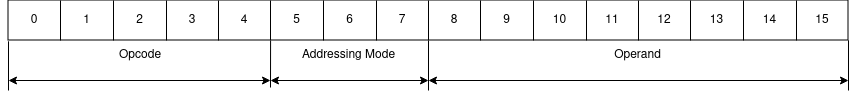
\includegraphics[scale=0.40]{img/Instruction_Format}
    \end{center}
    \par Instructions are divided into three fields, the opcode, addressing mode and operand fields.
    \begin{itemize}
        \item The Opcode Field (0-4): Indicates the operation to be performed on the data
        \item The Addressing Mode Field (5-7): Determines how the operand field will be used.
        The operand field can be used as an immediate value, or as an address to some other value in memory,
        depending on the addressing mode
        \item The Operand Field (8-15): An 8-bit constant that, in combination with the Addressing Mode Field, is
        used to determine the value to use in an operation.
    \end{itemize}

    \subsection{Representing Numbers}\label{subsec:representing-numbers}
    \par All values will be stored in two's complement form.
    Addition and subtraction will both be two's complement operations.


    \subsection{Reset Sequence}\label{subsec:reset-sequence}
    \par While the machine is in reset, the reset line on the bus will be held low.
    After exiting reset, the Accumulator, Instruction Register and Program Counter will
    be set to zero.
    The machine will then begin executing code at address $0000_{16}$.


    \subsection{Invalid Instruction Trap}\label{subsec:invalid-instruction-trap}
    \par Should the machine encounter an invalid instruction, the machine will execute a JSR to address $0002_{16}$.
    That is, a pointer to the next instruction will be loaded into the accumulator, and $0002_{16}$ will be loaded
    into the program counter.
    \pagebreak

    \section{Addressing Modes}\label{subsec:addressing-modes}
\par Any addressing mode can be applied to instructions that need a data source.
The addressing mode determines how that data will be obtained.

\subsection{Immediate}\label{subsec:immediate-(imm)}
\subsubsection{Syntax}
\begin{verbatim}[operation].imm [8-bit immediate]\end{verbatim}

\subsubsection{Description}
$OperandValue = SignExtend(Immediate)$
\par The 8-bit operand field will be sign-extended to 16-bits.
It will then immediately be used as the secondary operand for the instruction.

\subsubsection{Encoding}
\begin{center}
    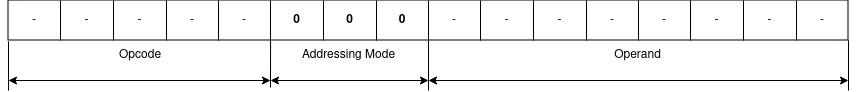
\includegraphics[scale=0.40]{img/Andromeda-IMM.drawio}
\end{center}

\subsubsection{Example}
\begin{verbatim}

        org(0x0000)
    def entry:
        lda.imm     -12
        hlt

\end{verbatim}
The code above would result in `-12' being loaded into the accumulator.
The 16-bit two's complement form of -12 is $1111111111110100_{2}$.
This value is the sign-extended version of the 8-bit value `$1111010_{2}$' that was embedded in the instruction's operand field.
\pagebreak

\subsection{Memory Direct}\label{subsec:memory-direct-(dir)}
\subsubsection{Syntax}
\begin{verbatim}[operation].dir [8-bit immediate]\end{verbatim}

\subsubsection{Description}
$OperandValue = Memory[FF00_{16} + Immediate]$
\par The constant $FF00_{16}$ will be added to the 8-bit operand field.
This will yield a 16-bit value in the range $FF00_{16}$ - $FFFF_{16}$ inclusive.
This value will then be used as an address.
The value stored at that address will be used as the secondary operand for the instruction.

\subsubsection{Encoding}
\begin{center}
    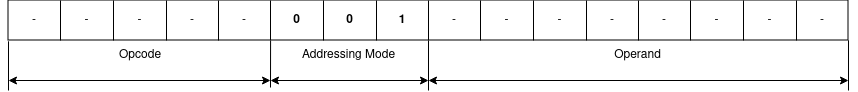
\includegraphics[scale=0.40]{img/Andromeda-DIR.drawio}
\end{center}

\subsubsection{Example}
\begin{verbatim}

        org(0x0000)
    def entry:
        sta.dir     0x01
        hlt

\end{verbatim}
The code above would store the accumulator into the address $FF01_{16}$.
\pagebreak

\subsection{Relative Memory Direct}\label{subsec:relative-direct-(rel)}

\subsubsection{Syntax}
\begin{verbatim}[operation].rel [8-bit immediate]\end{verbatim}

\subsubsection{Description}
$OperandValue = Memory[PC + SignExtend(Immediate)]$
\par The 8-bit operand field is sign-extended to 16-bits.
That value is added to the program counter (PC) to yield and address.
The contents of that address will be used as the secondary operand for the instruction.

\subsubsection{Encoding}
\begin{center}
    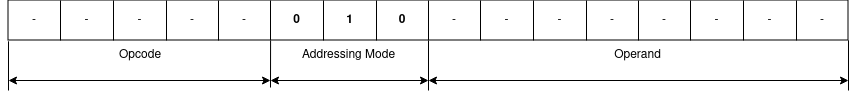
\includegraphics[scale=0.40]{img/Andromeda-REL.drawio}
\end{center}

\subsubsection{Example}
\begin{verbatim}

        org(0x0000)
    def entry:
        nop
        lda.rel     2
        hlt
    def data:
        dw(-11)

\end{verbatim}
The code above would be result in -11 being loaded into the Accumulator.
The `lda' instruction exists at address $0001_{16}$, adding `2' to this address results in the value $0003_{16}$.
The value stored at $0003_{16}$ (`-11') is loaded into the Accumulator.
\pagebreak

\subsection{Offset}\label{subsec:relative-jump}
\subsubsection{Syntax}
\begin{verbatim}[operation].off [8-bit immediate]\end{verbatim}

\subsubsection{Description}
$OperandValue = PC + SignExtend(Immediate)$
\par The 8-bit operand field is sign-extended to 16-bits.
That value is added to the program counter (PC) to yield the operand value.

\subsubsection{Encoding}
\begin{center}
    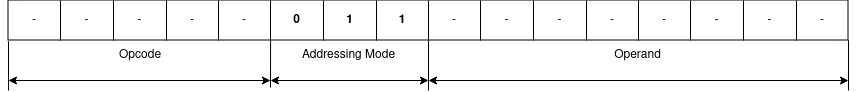
\includegraphics[scale=0.40]{img/Andromeda-OFF.drawio}
\end{center}

\subsubsection{Example}
\begin{verbatim}

    org(0x0000)
def entry:
    lda.imm     100
    jmp.off     2
    lda.imm     200
    hlt

\end{verbatim}
The code above would result in `$100_{10}$' in the Accumulator.
The \texttt{jmp.off 2} exists at address $0001_{16}$.
Adding $0002_{16}$ to that address results in address $0004_{16}$, where the halt instruction exists.
As a result, Tth \texttt{jmp.off 2} instruction skipped the `\texttt{lda.imm 200}' instruction.
This means only the first `\texttt{lda.imm 100}' instruction was executed.
\pagebreak

\subsection{Memory Indirect}\label{subsec:memory-indirect-(ind)}
\subsubsection{Syntax}
\begin{verbatim}[jump operation].ind [8-bit immediate]\end{verbatim}

\subsubsection{Description}
$OperandValue = Memory[Memory[FF00_{16} + Immediate]]$
\par The constant $FF00_{16}$ will be added to the 8-bit operand field.
This will yield a 16-bit value in the range $FF00_{16}$ - $FFFF_{16}$ inclusive.
This value will then be used as an address.
The value stored at that address will be used as another address known as the pointer.
This value stored at this final pointer address will be used as the secondary operand for the instruction.

\subsubsection{Encoding}
\begin{center}
    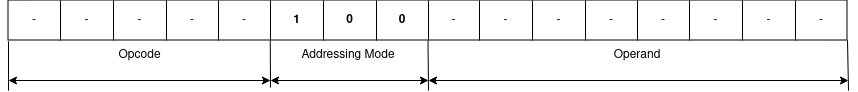
\includegraphics[scale=0.40]{img/Andromeda-IND.drawio}
\end{center}

\subsubsection{Example}
\begin{verbatim}

        org(0x0000)
    def entry:
        lda.ind pointer
        hlt

        org(0xFF01)
    def pointer:
        0xD000

        org(0xD000)
    def final_value:
        -12

\end{verbatim}
The code above will result in -12 being loaded into the accumulator.
The value stored in address $FF01_{16}$ ($D000_{16}$) was used as an address to find the final value (-12).
\pagebreak

\subsection{Memory Indirect \& Auto Increment}\label{subsec:memory-indirect-&-auto-increment-(inc)}
\subsubsection{Syntax}
\begin{verbatim}[jump operation].inc [8-bit immediate]\end{verbatim}

\subsubsection{Description}
$OperandValue = Memory[Memory[(FF00_{16} + Immediate)++]]$\\
\par This addressing mode behaves similarly to memory indirect addressing.
The secondary operand is obtained in the same manner.
However, after the value is obtained, the pointer will be incremented.

\subsubsection{Encoding}
\begin{center}
    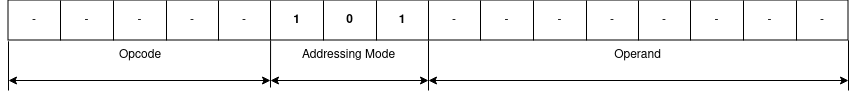
\includegraphics[scale=0.40]{img/Andromeda-INC.drawio}
\end{center}

\subsubsection{Example}
\begin{verbatim}

        org(0x0000)
    def entry:
        lda.inc pointer
        hlt

        org(0xFF01)
    def pointer:
        0xD000

        org(0xD000)
    def final_value:
        -12

\end{verbatim}
The code above will result in -12 being loaded into the accumulator.
However, after the instruction has completed execution, pointer will be incremented to $D001_{16}$
\pagebreak

\subsection{Auto Decrement \& Memory Indirect}\label{subsec:auto-decrement-&-memory-indirect-(dec)}
\subsubsection{Syntax}
\begin{verbatim}[jump operation].dec [8-bit immediate]\end{verbatim}

\subsubsection{Description}
$OperandValue = Memory[Memory[--(FF00_{16} + Immediate)]]$
\par This addressing mode behaves similarly to memory indirect addressing.
Before the instruction is executed, the pointer will be decremented.
Then the secondary operand is obtained in the same manner as it is in simple Memory Indirect addressing.

\subsubsection{Encoding}
\begin{center}
    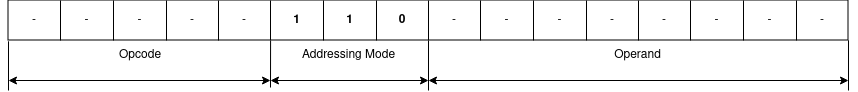
\includegraphics[scale=0.40]{img/Andromeda-DEC.drawio}
\end{center}

\subsubsection{Example}
\begin{verbatim}

        org(0x0000)
    def entry:
        lda.dec pointer
        hlt

        org(0xFF01)
    def pointer:
        0xD001

        org(0xD000)
    def final_value:
        13
        -12

\end{verbatim}
The code above will result in 13 being loaded into the accumulator.
Pointer will have been decremented to $D000_{16}$ so the `13' could be addressed indirectly
\pagebreak

\subsection{Reference Card}\label{subsec:reference-card}
\renewcommand{\arraystretch}{2.0}
\begin{center}
    \begin{adjustbox}{width=\textwidth}
        \begin{tabular}{ |c|c|c| }
            \hline
            Mnemonic & Operand Value & Encoding \\ \hline
            \texttt{imm} & $SignExtend(Immediate)$ & $000_{2}$ \\ \hline
            \texttt{dir} & $Memory[FF00_{16} + Immediate]$ & $001_{2}$\\ \hline
            \texttt{rel} & $Memory[PC + SignExtend(Immediate)]$ & $010_{2}$\\ \hline
            \texttt{off} & $PC + SignExtend(Immediate)$ & $011_{2}$\\ \hline
            \texttt{ind} & $Memory[Memory[FF00_{16} + Immediate]]$ & $100_{2}$\\ \hline
            \texttt{inc} & $Memory[Memory[(FF00_{16} + Immediate)++]]$ & $101_{2}$\\ \hline
            \texttt{dec} & $Memory[--(Memory[FF00_{16} + Immediate)]]$ & $110_{2}$\\ \hline
        \end{tabular}
    \end{adjustbox}
\end{center}

Note: The table above uses the C/C++ convention for postfixing and prefixing increments (\texttt{++}) and decrements (\texttt{--}).
\par If the operator appears before the value, the operation is performed before the value is calculated.
If the operator appears after the value, the operation is performed after the value is calculated.

    \pagebreak
    \subsection{LDA}\label{subsec:lda}
    \subsubsection{Description}
    $Accumulator \leftarrow Operand Value$
    \par Load the value indicated by the operand and addressing mode fields into the Accumulator.

    \subsubsection{Encoding}

    \subsubsection{Process}
    \begin{enumerate}
        \item
    \end{enumerate}

    \subsubsection{Example}
    \begin{verbatim}
        org(0x0000)
    def entry:
        lda.dir     data

        org(0xFF01)
    def data:
        dw(-11)
    \end{verbatim}
    \par The above code would result in `-11' being loaded into the Accumulator.


\subsection{STA}\label{subsec:sta}
    \subsubsection{Description}
    $if\ (AddressingMode \neq IMM)\ \{ *OperandValue \leftarrow Accumulator \}$ \\
    $else\ \{ *Accumulator \leftarrow OperandValue \}$
    \par If the addressing mode is not `imm,' then store the contents of the accumulator into the address indicated by
    the operand value.
    If the addressing mode is `imm,' the operand value is loaded into the address indicated by the Accumulator.

    \subsubsection{Encoding}
    \subsubsection{Process}
    \begin{enumerate}
        \item
    \end{enumerate}

    \subsubsection{Example}
    \begin{verbatim}
    \end{verbatim}

\subsection{ADD}\label{subsec:add}
    \subsubsection{Description}
    $Accumulator \leftarrow Accumulator + OperandValue$
    \par Add the contents of the Accumulator, and the value indicated by the operand and addressing fields.
    Store the result in the Accumulator.

    \subsubsection{Encoding}
    \subsubsection{Process}
    \begin{enumerate}
        \item
    \end{enumerate}

    \subsubsection{Example}
    \begin{verbatim}
    \end{verbatim}

\subsection{SUB}\label{subsec:sub}
    \subsubsection{Description}
    $Accumulator \leftarrow Accumulator - OperandValue$
    \par Subtract the value indicated by the operand and addressing fields from the contents of the Accumulator.
    Store the result in the Accumulator.

    \subsubsection{Encoding}
    \subsubsection{Process}
    \begin{enumerate}
        \item
    \end{enumerate}

    \subsubsection{Example}
    \begin{verbatim}
    \end{verbatim}

\subsection{XOR}\label{subsec:xor}
    \subsubsection{Description}
    $Accumulator \leftarrow Accumulator \oplus OperandValue$
    \par Exclusive or the contents of the Accumulator, and the value indicated by the operand and addressing fields.
    Store the result in the Accumulator.

    \subsubsection{Encoding}
    \subsubsection{Process}
    \begin{enumerate}
        \item
    \end{enumerate}

    \subsubsection{Example}
    \begin{verbatim}
    \end{verbatim}

\subsection{NND}\label{subsec:nand}
    \subsubsection{Description}
    $Accumulator \leftarrow \overline{Accumulator \land OperandValue}$
    \par Nand the contents of the Accumulator, and the value indicated by the operand and addressing fields.
    Store the result in the Accumulator.

    \subsubsection{Encoding}
    \subsubsection{Process}
    \begin{enumerate}
        \item
    \end{enumerate}

    \subsubsection{Example}
    \begin{verbatim}
    \end{verbatim}

\subsection{JMP}\label{subsec:jmp}
    \subsubsection{Description}
    $PC \leftarrow OperandValue$
    \par Load the value indicated by the operand and addressing fields into the program counter.
    \subsubsection{Encoding}
    \subsubsection{Process}
    \begin{enumerate}
        \item
    \end{enumerate}

    \subsubsection{Example}
    \begin{verbatim}
    \end{verbatim}

\subsection{JSR}\label{subsec:jsr}
    \subsubsection{Description}
    $Accumulator \leftarrow PC$; $PC \leftarrow OperandValue$
    \par Load the program counter into the Accumulator.
    Load the operand value into the program counter.
    \subsubsection{Encoding}
    \subsubsection{Process}
    \begin{enumerate}
        \item
    \end{enumerate}

    \subsubsection{Example}
    \begin{verbatim}
    \end{verbatim}

\subsection{JNS}\label{subsec:jns}
    \subsubsection{Description}
    $if\ (Accumulator \geq 0)\ \{ PC \leftarrow OperandValue \}$
    \par If the contents of the Accumulator are greater than, or equal to, zero, load the operand value into the PC\@.
    \subsubsection{Encoding}
    \subsubsection{Process}
    \begin{enumerate}
        \item
    \end{enumerate}

    \subsubsection{Example}
    \begin{verbatim}
    \end{verbatim}

\subsection{JNZ}\label{subsec:jnz}
    \subsubsection{Description}
    $if\ (Accumulator \neq 0)\ \{ PC \leftarrow OperandValue \}$
    \par If the contents of the Accumulator are not equal to zero, load the operand value into the PC\@.
    \subsubsection{Encoding}
    \subsubsection{Process}
    \begin{enumerate}
        \item
    \end{enumerate}

    \subsubsection{Example}
    \begin{verbatim}
    \end{verbatim}

\subsection{HALT}\label{subsec:halt}
    \subsubsection{Description}
    $HFF \leftarrow 1$
    \par Stop the system clock by setting the halt flip-flop.
    \subsubsection{Encoding}
    \subsubsection{Process}
    \begin{enumerate}
        \item
    \end{enumerate}

    \subsubsection{Example}
    \begin{verbatim}
    \end{verbatim}

\subsection{NOP}\label{subsec:nop}
    \subsubsection{Description}
    $ -- $
    \par Continue to the next instruction without changing the machine's state.
    \subsubsection{Encoding}
    \subsubsection{Process}
    \begin{enumerate}
        \item
    \end{enumerate}

    \subsubsection{Example}
    \begin{verbatim}
    \end{verbatim}
    \section{Control Algorithm}\label{sec:abstract-description}
\subsection{Block Diagram}\label{subsec:block-diagram}
\begin{center}
    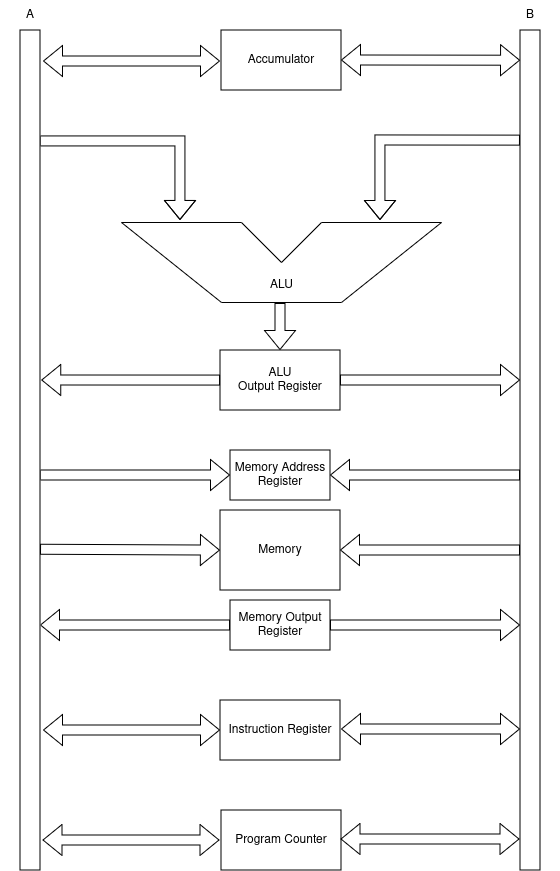
\includegraphics[scale=0.58]{img/Andromeda-Block Diagram.drawio}
\end{center}

\subsection{Instruction Flow}\label{subsec:state-machine-diagrams}
\par This section outlines the algorithm each instruction/addressing mode pair will execute.
The algorithm is laid out in terms of what steps will be executed for every rising and falling edge of the system clock.
Each step will correspond to a single micro-instruction.

\pagebreak
\subsubsection{\texttt{lda.imm}}
\subsubsection{\texttt{lda.dir}}
\subsubsection{\texttt{lda.rel}}
\subsubsection{\texttt{lda.off}}
\subsubsection{\texttt{lda.ind}}
\subsubsection{\texttt{lda.inc}}
\subsubsection{\texttt{lda.dec}}

\subsubsection{\texttt{sta.imm}}
\subsubsection{\texttt{sta.dir}}
\subsubsection{\texttt{sta.rel}}
\subsubsection{\texttt{sta.off}}
\subsubsection{\texttt{sta.ind}}
\subsubsection{\texttt{sta.inc}}
\subsubsection{\texttt{sta.dec}}

\subsubsection{\texttt{add.imm}}
\subsubsection{\texttt{add.dir}}
\subsubsection{\texttt{add.rel}}
\subsubsection{\texttt{add.off}}
\subsubsection{\texttt{add.ind}}
\subsubsection{\texttt{add.inc}}
\subsubsection{\texttt{add.dec}}

\subsubsection{\texttt{xor.imm}}
\subsubsection{\texttt{xor.dir}}
\subsubsection{\texttt{xor.rel}}
\subsubsection{\texttt{xor.off}}
\subsubsection{\texttt{xor.ind}}
\subsubsection{\texttt{xor.inc}}
\subsubsection{\texttt{xor.dec}}


    \section{Hardware}\label{sec:hardware}
    \section{Forth Environment}\label{sec:forth-environment}
The Andromeda comes with a minimal forth environment in ROM.
This serves as a primative operating system and programming environment.

\subsection{Words}\label{subsec:implemented-words}
The forth environment implements a small subset of ANS Forth, as well as the optional `block' word set.
These words are outlined below.
For more information on how to program in Forth, consult outside sources on the subject.
\begin{center}
    \newcolumntype{P}[1]{>{\centering\arraybackslash}p{#1}}
    \begin{longtable}{|P{0.13\linewidth}|P{0.07\linewidth}|P{0.12\linewidth}|P{0.17\linewidth}|P{0.45\linewidth}|}
            \hline
            Section & Symbol & Name & Stack Effects & Description \\
            \hline
            6.1.0010 & \texttt{!} & ``store" & \texttt{(x a-addr -- )} & Store the value `x' at the address `a-addr.' \\
            \hline
            6.1.0150 & \texttt{,} & ``comma" & \texttt{(x -- )} & Reserve one cell of data space and store `x' in the cell. \\
            \hline
            6.1.650 & \texttt{@} & ``fetch" & \texttt{(a-addr -- x)} & x is the value stored in `a-addr.' \\
            \hline
            6.1.0120 & \texttt{+} & ``plus" & \texttt{(n1 n2 -- n3)} & Add \texttt{n1} and \texttt{n2}, giving \texttt{n3} as the sum \\
            \hline
            6.1.0090 & \texttt{*} & ``star" & \texttt{(n1 n2 -- n3)} & Multiply \texttt{n1} and \texttt{n2}, giving \texttt{n3} as the product \\
            \hline
            6.1.0320 & \texttt{2*} & ``two-star" & \texttt{(n1 -- n2)} & Shift \texttt{n1} left, filling the vacated bit with a zero \\
            \hline
            6.1.0160 & \texttt{-} & ``minus" & \texttt{(n1 n2 -- n3)} & Subtract \texttt{n1} and \texttt{n2}, giving \texttt{n3} as the difference\\
            \hline
            6.1.0240 & \texttt{/mod} & ``slash-mod" & \texttt{(n1 n2 -- n3 n4)} & Divide \texttt{n1} by \texttt{n2}, giving remainder as \texttt{n3},and the quotient as \texttt{n4}\\
            \hline
            6.1.0230 & \texttt{/} & ``slash" & \texttt{(n1 n2 -- n3)} & Divide \texttt{n1} by \texttt{n2}, giving \texttt{n3} as the quotient\\
            \hline
            6.1.0330 & \texttt{2/} & ``two-slash" & \texttt{(x1 -- x2)} & \texttt{x2} is the result of shifting \texttt{x1} one bit right, leaving the most significant bit unchanged \\
            \hline
            6.1.1890 & \texttt{mod} & ``mod" & \texttt{(n1 n2 -- n3)} & Divide \texttt{n1} by \texttt{n2}, giving the remainder \texttt{n3} \\
            \hline
            6.1.0270 & \texttt{0=} & ``zero-equals" & \texttt{(x -- flag)} & Flag is true if and only if x is equal to zero \\
            \hline
            6.1.0250 & \texttt{0<} & ``zero-less" & \texttt{(n -- flag)} & Flag is true if and only if x is less than zero \\
            \hline
            6.1.0720 & \texttt{\&} & ``and" & \texttt{(x1 x2 -- x3)} & \texttt{x3} is the bitwise logical ``and" of \texttt{x1} and \texttt{x2} \\
            \hline
            6.1.1720 & \texttt{invert} & ``invert" & \texttt{(x1 -- x2)} & \texttt{x2} is the bitwise logical inverse of \texttt{x1} \\
            \hline
            6.2.2298 & \texttt{true} & ``true" & \texttt{( -- true)} & Return a `true' flag, a single-celled value with all bits set \\
            \hline
            6.2.1485 & \texttt{false} & ``false" & \texttt{( -- false)} & Return a `false' flag, a single-celled value with all bits unset \\
            \hline
            6.1.0530 & \texttt{=} & ``equals" & \texttt{(x1 x2 -- flag)} & Flag is true if and only if \texttt{x1} is bit-for-bit the same as \texttt{x2} \\
            \hline
            6.1.0540 & \texttt{>} & ``greater-than" & \texttt{(n1 n2 -- flag)} & Flag is true if and only if \texttt{n1} is greater than \texttt{n2} \\
            \hline
            6.1.2490 & \texttt{xor} & ``x-or" & \texttt{(x1 x2 -- x3)} & \texttt{x3} is the bitwise exclusive-or of \texttt{x1} with \texttt{x2} \\
            \hline
            6.1.1290 & \texttt{dup} & ``dupe" & \texttt{(x -- x x)} & Duplicate \texttt{x}\\
            \hline
            6.1.2260 & \texttt{swap} & ``swap" & \texttt{(x1 x2 -- x2 x1)} & Exchange the top two stack items \\
            \hline
            6.1.1290 & \texttt{drop} & ``drop" & \texttt{(x -- )} & Remove \texttt{x} from the stack \\
            \hline
            6.1.1990 & \texttt{over} & ``over" & \texttt{(x1 x2 -- x1 x2 x1)} & Place a copy of \texttt{x1} on top of the stack \\
            \hline
            6.1.2160 & \texttt{rot} & ``rote" & \texttt{(x1 x2 x3 -- x2 x3 x1)} & Rotate the top three stack entries \\
            \hline
            6.1.0580 & \texttt{>R} & ``to-r" & \texttt{(x -- ) R:( -- x)} & Move \texttt{x} to the return stack \\
            \hline
            6.1.2070 & \texttt{R@} & ``r-fetch" & \texttt{( -- x) R:(x -- x)} & Copy \texttt{x} from the return stack to the data stack \\
            \hline
            6.1.2060 & \texttt{R>} & ``r-from" & \texttt{( -- x) R:(x -- )} &  Move \texttt{x} from the return stack to the data stack \\
            \hline
            6.1.1750 & \texttt{key} & ``key" & \texttt{( -- char)} & Read an input character, place it on the stack \\
            \hline
            6.1.1320 & \texttt{emit} & ``emit" & \texttt{(x -- )} & Write a character to the display \\
            \hline
            10.6.1.1755 & \texttt{key?} & ``key-question" & \texttt{( -- flag)} & Flat is \texttt{true} if and only if a character is ready to be read \\
            \hline
            6.1.0990 & \texttt{cr} & ``c-r" & \texttt{( -- )} & Write a carraige return to the display \\
            \hline
            15.6.1.0220 & \texttt{.s} & ``dot-s" & \texttt{( -- )} & Copy and display the values currently on the data stack \\
            \hline
            6.1.1700 & \texttt{if} & ``if" & \texttt{(x -- )} & If all bits of \texttt{x} are zero, skip forward to the next ``then" or ``else" token \\
            \hline
            6.1.2270 & \texttt{then} & ``then" & \texttt{( -- )} & Continue execution \\
            \hline
            6.1.1310 & \texttt{else} & ``else" & \texttt{( -- )} & Jump target point when ``if" evaluates false \\
            \hline
            6.1.2430 & \texttt{while} & ``while" & \texttt{(flag -- )} & If flag is true, continue. If flag is false, terminate the loop (after \texttt{REPEAT}) \\
            \hline
        \end{longtable}
\end{center}


\subsubsection{Repeat}
\subsubsection{Do}
\subsubsection{I}
\subsubsection{Tick}
\subsubsection{Begin}
\subsubsection{Again}
\subsubsection{Until}
\subsubsection{Loop}
\subsubsection{J}

\subsubsection{Execute}
\subsubsection{Colon}
\subsubsection{Constant}
\subsubsection{Create}
\subsubsection{Semicolon}
\subsubsection{Variable}
\subsubsection{Does}

\subsubsection{Paren}
\subsubsection{Backslash}

\subsubsection{Block}
\subsubsection{Buffer}
\subsubsection{Load}
\subsubsection{List}
\subsubsection{Through}



\end{document}